%%%%%%%%%%%%%%%%%%%%%%%%%%%%%%%%%%%%%%%%%%%%%%%%%%%%%%%%%%%%%%%%%%%%%%%%
% Chapter: Differential Dynamic Programming for MPOPF
% Context: Temporal decomposition via DDP
%%%%%%%%%%%%%%%%%%%%%%%%%%%%%%%%%%%%%%%%%%%%%%%%%%%%%%%%%%%%%%%%%%%%%%%%
\clearpage
\section{Temporal Decomposition via Differential Dynamic Programming}
\label{sec:ddp}

%%%%%%%%%%%%%%%%%%%%%%%%%%%%%%%%%%%%%%%%%%%%%%%%%%%%%%%%%%%%%%%%%%%%%%%%
\subsection{Introduction}
%%%%%%%%%%%%%%%%%%%%%%%%%%%%%%%%%%%%%%%%%%%%%%%%%%%%%%%%%%%%%%%%%%%%%%%%

While the spatial decomposition approach (ENApp) demonstrated in \Cref{sec:enapp} effectively partitions the network topology, it encounters computational challenges for long time horizons due to the temporal coupling through battery state-of-charge (SOC) dynamics. As shown in the previous chapter, spatial decomposition alone remains computationally expensive for planning horizons exceeding 10 hours.

This motivates the investigation of \textbf{temporal decomposition} methods that can break down the multi-period optimization problem across time while maintaining feasibility and near-optimality. One such approach is \textbf{Differential Dynamic Programming (DDP)} \cite{ddp_sugar_01}, which leverages the sequential structure of the MPOPF problem to decompose it into a backward-forward sweep algorithm.

DDP offers several advantages for MPOPF:
\begin{itemize}
    \item \textbf{Temporal Decomposition}: Solves single-period subproblems sequentially
    \item \textbf{Handles Nonlinearity}: Can work with nonlinear branch flow models (BFM-NL) without requiring linearization
    \item \textbf{Scalability}: Computational complexity grows linearly with time horizon length
    \item \textbf{Local Optimality}: Guarantees convergence to local optima through iterative refinement
    \item \textbf{Guaranteed Feasibility always}: At any Forward Pass iteration ensures that its current solution is feasible (provided there are no terminal constraints on state variable such as terminal SOC constraint)
\end{itemize}

%%%%%%%%%%%%%%%%%%%%%%%%%%%%%%%%%%%%%%%%%%%%%%%%%%%%%%%%%%%%%%%%%%%%%%%%
\subsection{DDP Algorithm for MPOPF}
%%%%%%%%%%%%%%%%%%%%%%%%%%%%%%%%%%%%%%%%%%%%%%%%%%%%%%%%%%%%%%%%%%%%%%%%

The DDP algorithm iteratively refines a nominal trajectory through backward-forward sweeps. For MPOPF, the algorithm proceeds as follows:

\subsubsection*{DDP Workflow: Forward Pass for Non-Terminal Time-Step $t \in \{1, 2, \ldots T-1\}$}

At each non-terminal time-step, the forward pass solves the following optimization problem where the previous battery SOC $\textcolor{red}{B_{j}^{t-1}}$ is known from the previous time-step, and the Lagrange multiplier $\textcolor{blue}{\mu_{SOC{_j}}^{t+1}}$ from the next time-step influences the current decision:

\begin{gather}
    \begin{align}
        \min_{} 
        \vspace{-15ex}
        & \quad
        C^t P_{Subs}^t \\
        &+ \alpha \sum_{j \in \mathcal{B}} \left\{ (1- \eta_c)P_{c_j}^t + \left(\frac{1}{\eta_d}-1\right) P_{d_j}^t \right\} \nonumber\\
        &+ \sum_{j \in \mathcal{B}} { \textcolor{blue}{ \mu_{SOC{_j}}^{t+1}} \left\{ - B_{j}^{t} \right\} } \nonumber\\
        \text{s.t.} & {}\nonumber\\
        {0} & = {\sum_{(j, k) \in \mathcal{L}} \left\{P_{jk}^t\right\} - \left\{P_{ij}^t - r_{ij}l_{ij}^t\right\} - (P_{d_j}^t - P_{c_j}^t)  - (p_D{_j}^t) + p_L{_j}^t} && \\
        {0} & = {\sum_{(j, k) \in \mathcal{L}} \left\{Q_{jk}^t\right\} - \left\{Q_{ij}^t - x_{ij}l_{ij}^t\right\} - (q_{D_j}^t) - (q_{B_j}^t) + q_L{_j}^t} && \\
        {0} & = {v_{i}^t - v_{j}^t - 2(r_{ij}P_{ij}^t + x_{ij}Q_{ij}^t) + \left\{r_{ij}^2 + x_{ij}^2\right\}l_{ij}^t}  && \\
        {0} & = {(P_{ij}^{t})^2 + (Q_{ij}^{t})^2 - v_{i}^t l_{ij}^t } \\
        {0} & = {B_{j}^{t} - \left\{ \textcolor{red}{ B_{j}^{t-1} } + \Delta t  \eta_c P_{c_j}^t - \Delta t\frac{1}{\eta_d} P_{d_j}^t \right\} } \\
        {0} & \geq {B{_{min_{j}}}^t - B{_j}^t} \\
        {0} & \geq {B{_j}^t - B{_{Max_{j}}}^t} \\
        {0} & \geq {\text{All other inequality constraints}}
    \end{align}
\end{gather}

\subsubsection*{DDP Workflow: Forward Pass for the Terminal Time-Step $t = T$}

At the terminal time-step, the forward pass includes the terminal penalty on battery SOC deviation from reference:

\begin{gather}
    \begin{align}
        \min_{} 
        \vspace{-15ex}
        & \quad
        C^t P_{Subs}^t \\
        &+ \alpha \sum_{j \in \mathcal{B}} \left\{ (1- \eta_c)P_{c_j}^t + \left(\frac{1}{\eta_d}-1\right) P_{d_j}^t \right\} \nonumber\\
        &+ \gamma \sum_{j \in \mathcal{B}} \left\{ \left(B^{T}_{j} - B_{ref_{j}}\right)^2\right\} \nonumber\\
        \text{s.t.} & {}\nonumber\\
        {0} & = {\sum_{(j, k) \in \mathcal{L}} \left\{P_{jk}^t\right\} - \left\{P_{ij}^t - r_{ij}l_{ij}^t\right\} - (P_{d_j}^t - P_{c_j}^t)  - (p_D{_j}^t) + p_L{_j}^t} && \\
        {0} & = {\sum_{(j, k) \in \mathcal{L}} \left\{Q_{jk}^t\right\} - \left\{Q_{ij}^t - x_{ij}l_{ij}^t\right\} - (q_{D_j}^t) - (q_{B_j}^t) + q_L{_j}^t} && \\
        {0} & = {v_{i}^t - v_{j}^t - 2(r_{ij}P_{ij}^t + x_{ij}Q_{ij}^t) + \left\{r_{ij}^2 + x_{ij}^2\right\}l_{ij}^t}  && \\
        {0} & = {(P_{ij}^{t})^2 + (Q_{ij}^{t})^2 - v_{i}^t l_{ij}^t } \\
        {0} & = {B_{j}^{t} - \left\{ \textcolor{red}{ B_{j}^{t-1} } + \Delta t  \eta_c P_{c_j}^t - \Delta t\frac{1}{\eta_d} P_{d_j}^t \right\} } \\
        {0} & \geq {B{_{min_{j}}}^t - B{_j}^t} \\
        {0} & \geq {B{_j}^t - B{_{Max_{j}}}^t} \\
        {0} & \geq {\text{All other inequality constraints}}
    \end{align}
\end{gather}

%%%%%%%%%%%%%%%%%%%%%%%%%%%%%%%%%%%%%%%%%%%%%%%%%%%%%%%%%%%%%%%%%%%%%%%%
\subsection{Computational Advantages for Long-Horizon MPOPF}
%%%%%%%%%%%%%%%%%%%%%%%%%%%%%%%%%%%%%%%%%%%%%%%%%%%%%%%%%%%%%%%%%%%%%%%%

DDP offers significant computational benefits compared to monolithic MPOPF formulations:

\begin{enumerate}        
    \item \textbf{Parallelizable Forward Pass}: Subproblems within forward pass can be solved in parallel across time steps.
    
    \item \textbf{Handles Nonlinearity}: Works directly with BFM-NL \cite{Farivar1} without requiring convex relaxations or linear approximations that may sacrifice accuracy.
    
    \item \textbf{Warm Starting}: Previous solutions provide excellent initialization for rolling-horizon Model Predictive Control (MPC) implementations.
\end{enumerate}

For MPOPF, the projection approach is most practical, as it maintains power flow feasibility explicitly.

%%%%%%%%%%%%%%%%%%%%%%%%%%%%%%%%%%%%%%%%%%%%%%%%%%%%%%%%%%%%%%%%%%%%%%%%
\subsection{Relationship to Other Decomposition Methods}
%%%%%%%%%%%%%%%%%%%%%%%%%%%%%%%%%%%%%%%%%%%%%%%%%%%%%%%%%%%%%%%%%%%%%%%%

DDP provides complementary capabilities to the spatial decomposition (ENApp, \Cref{sec:enapp}):

\begin{itemize}
    \item \textbf{ENApp}: Decomposes across \textit{space} (network topology), coupling through boundary voltage and power variables
    \item \textbf{DDP}: Decomposes across \textit{time} (temporal horizon), coupling through battery SOC evolution
    \item \textbf{Combined Approach}: Apply spatial decomposition (ENApp) within each DDP time-step subproblem, achieving both spatial and temporal scalability
\end{itemize}

Compared to ADMM-based temporal decomposition (next chapter):
\begin{itemize}
    \item \textbf{DDP}: Sequential backward-forward sweeps, local convergence to stationary points, guaranteed feasible solution at any stage of the algorithm
    \item \textbf{tADMM}: Parallel consensus-based optimization, handles separable structure, global convergence guarantees for convex problems, no guarantee of feasible solution at any current algorithm stage
    \item \textbf{Trade-off}: DDP more efficient for few iterations (warm start), ADMM more parallelizable for cold start
\end{itemize}

%%%%%%%%%%%%%%%%%%%%%%%%%%%%%%%%%%%%%%%%%%%%%%%%%%%%%%%%%%%%%%%%%%%%%%%%
\subsection{Numerical Results: 24-Hour Horizon on IEEE 123-Bus System}
%%%%%%%%%%%%%%%%%%%%%%%%%%%%%%%%%%%%%%%%%%%%%%%%%%%%%%%%%%%%%%%%%%%%%%%%

To demonstrate the effectiveness of DDP for temporal decomposition, we present results for a 24-hour planning horizon on the IEEE 123-bus single-phase equivalent system with 20\% PV penetration (31\% of buses with batteries). The system is optimized using the nonlinear Branch Flow Model (BFM-NL) with Ipopt solver.

\subsubsection{System Configuration and Convergence}

\Cref{fig:ddp-input-curves} shows the forecast curves for load, PV generation, and electricity cost over the 24-hour horizon. The load exhibits typical residential patterns with morning and evening peaks. PV generation follows solar irradiance with peak output during midday hours. Electricity costs vary throughout the day, with higher prices during peak demand periods.

\begin{figure}[h]
    \centering
    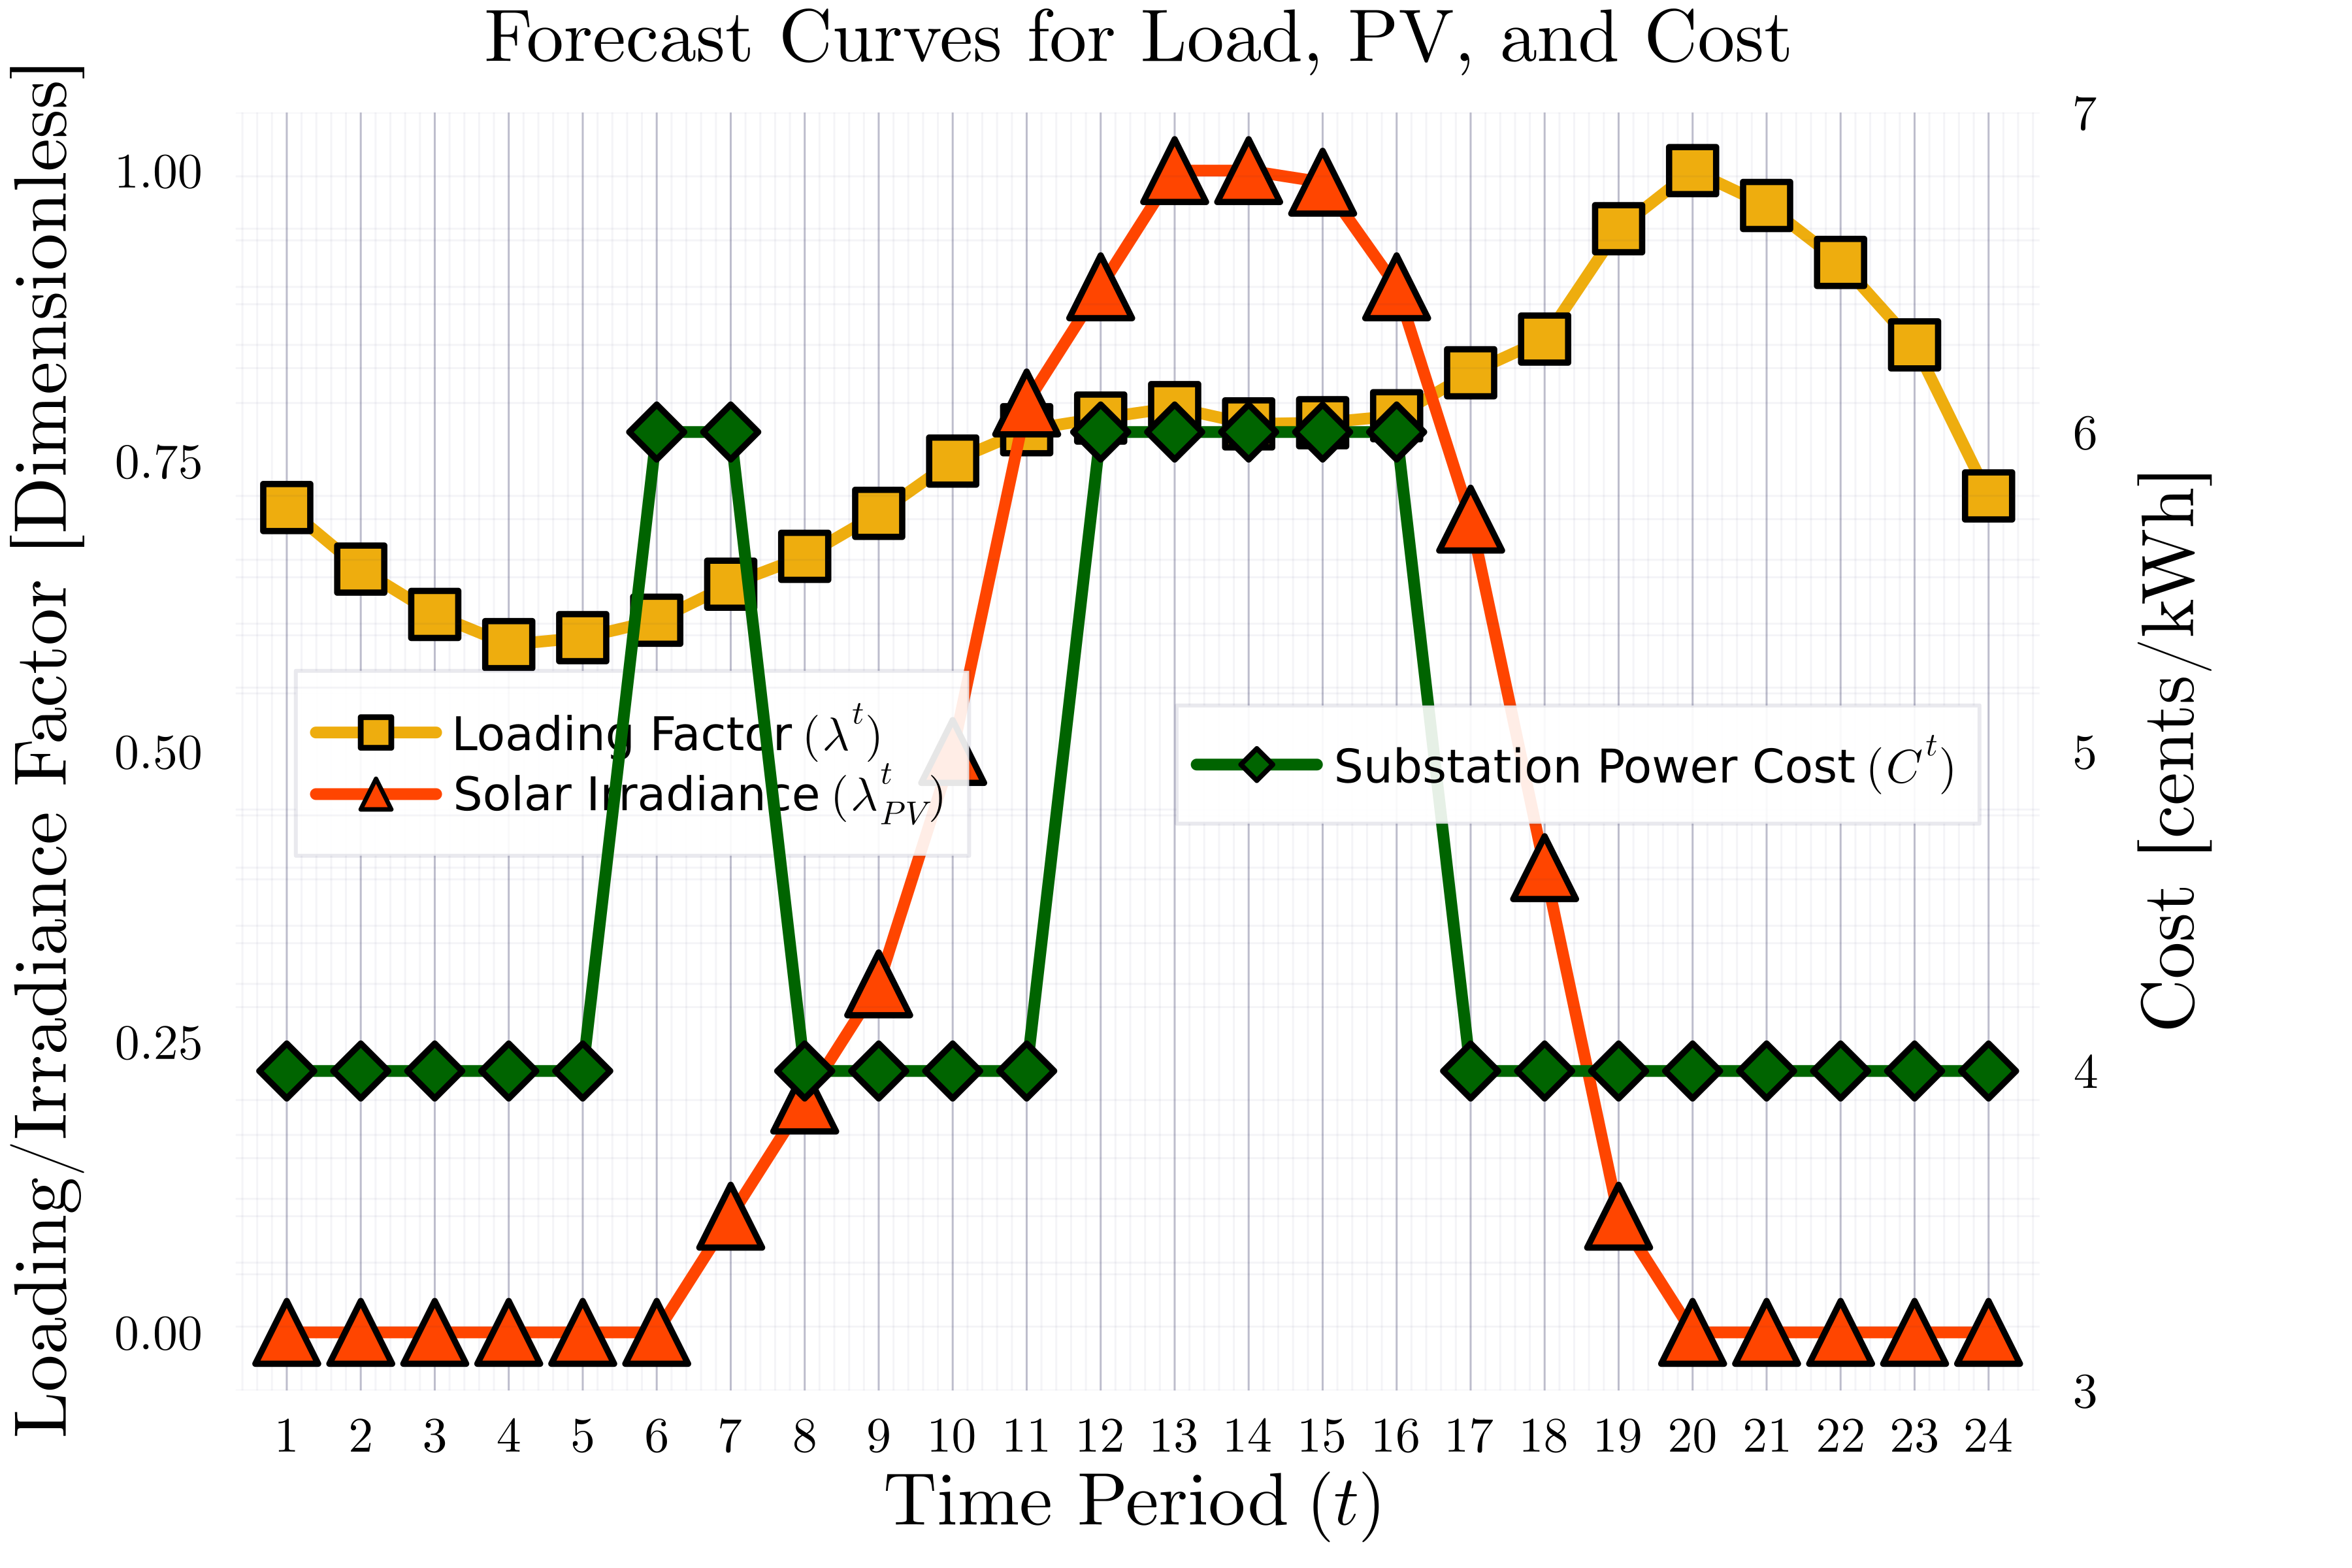
\includegraphics[width=0.85\textwidth]{figures/Horizon_24_InputForecastCurves_bilevelCosts.png}
    \caption{Forecast curves for loading factor ($\lambda^t$), solar irradiance ($\lambda_{PV}^t$), and substation power cost ($C^t$) over the 24-hour horizon.}
    \label{fig:ddp-input-curves}
\end{figure}

\Cref{fig:ddp-convergence-bfm,fig:ddp-convergence-ldf} present the convergence behavior of DDP compared to the temporally brute-forced (monolithic) approach for both BFM-NL and LinDistFlow models. The DDP algorithm demonstrates rapid convergence, achieving near-optimal solutions within 4-5 forward passes. After this initial rapid descent phase, the algorithm continues to refine the solution through additional iterations.

\begin{figure}[h]
    \centering
    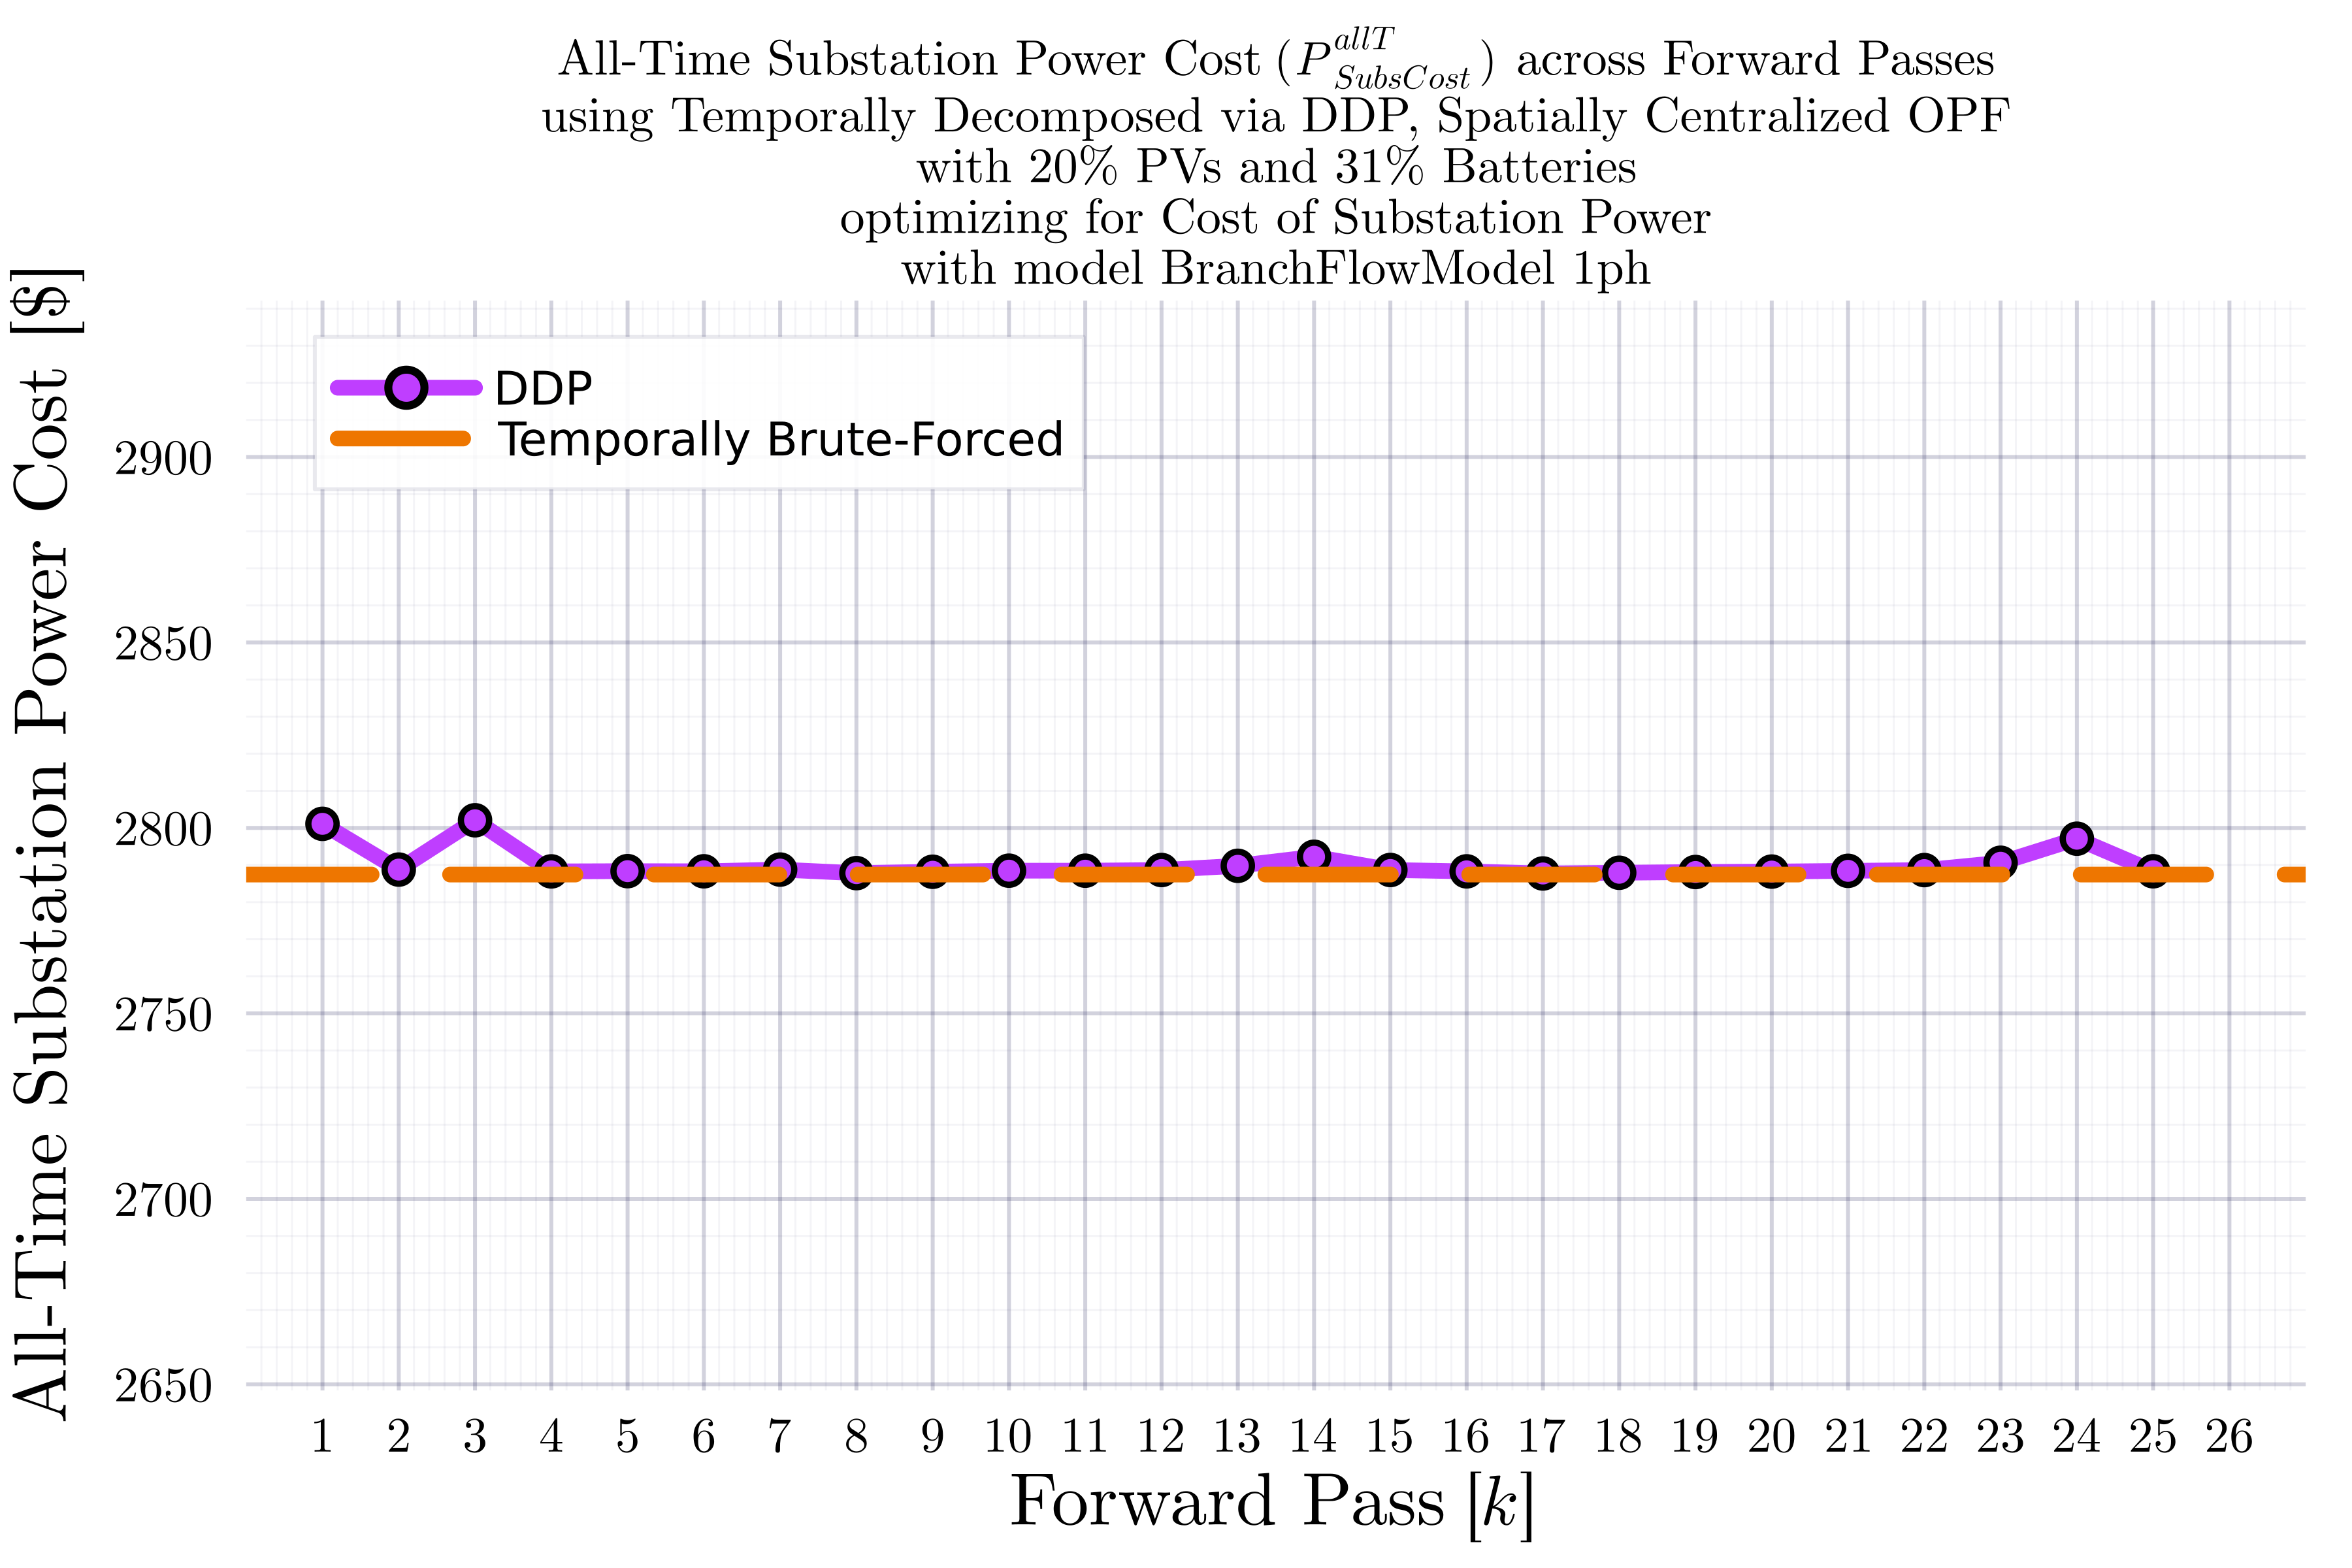
\includegraphics[width=0.85\textwidth]{figures/SubstationPowerCostAllTime_vs_k_26_for_subsPowerCost_min_with_scd_alpha_8_994_gamma_0_0_via_tmprl_dcmpsd_spat_centr_system_with_bfm_NL_1ph.png}
    \caption{All-time substation power cost convergence across forward passes using temporally decomposed DDP with spatially centralized formulation. BFM-NL model with 20\% PVs and 31\% batteries. DDP converges to the brute-forced solution within 4-5 iterations.}
    \label{fig:ddp-convergence-bfm}
\end{figure}

\begin{figure}[h]
    \centering
    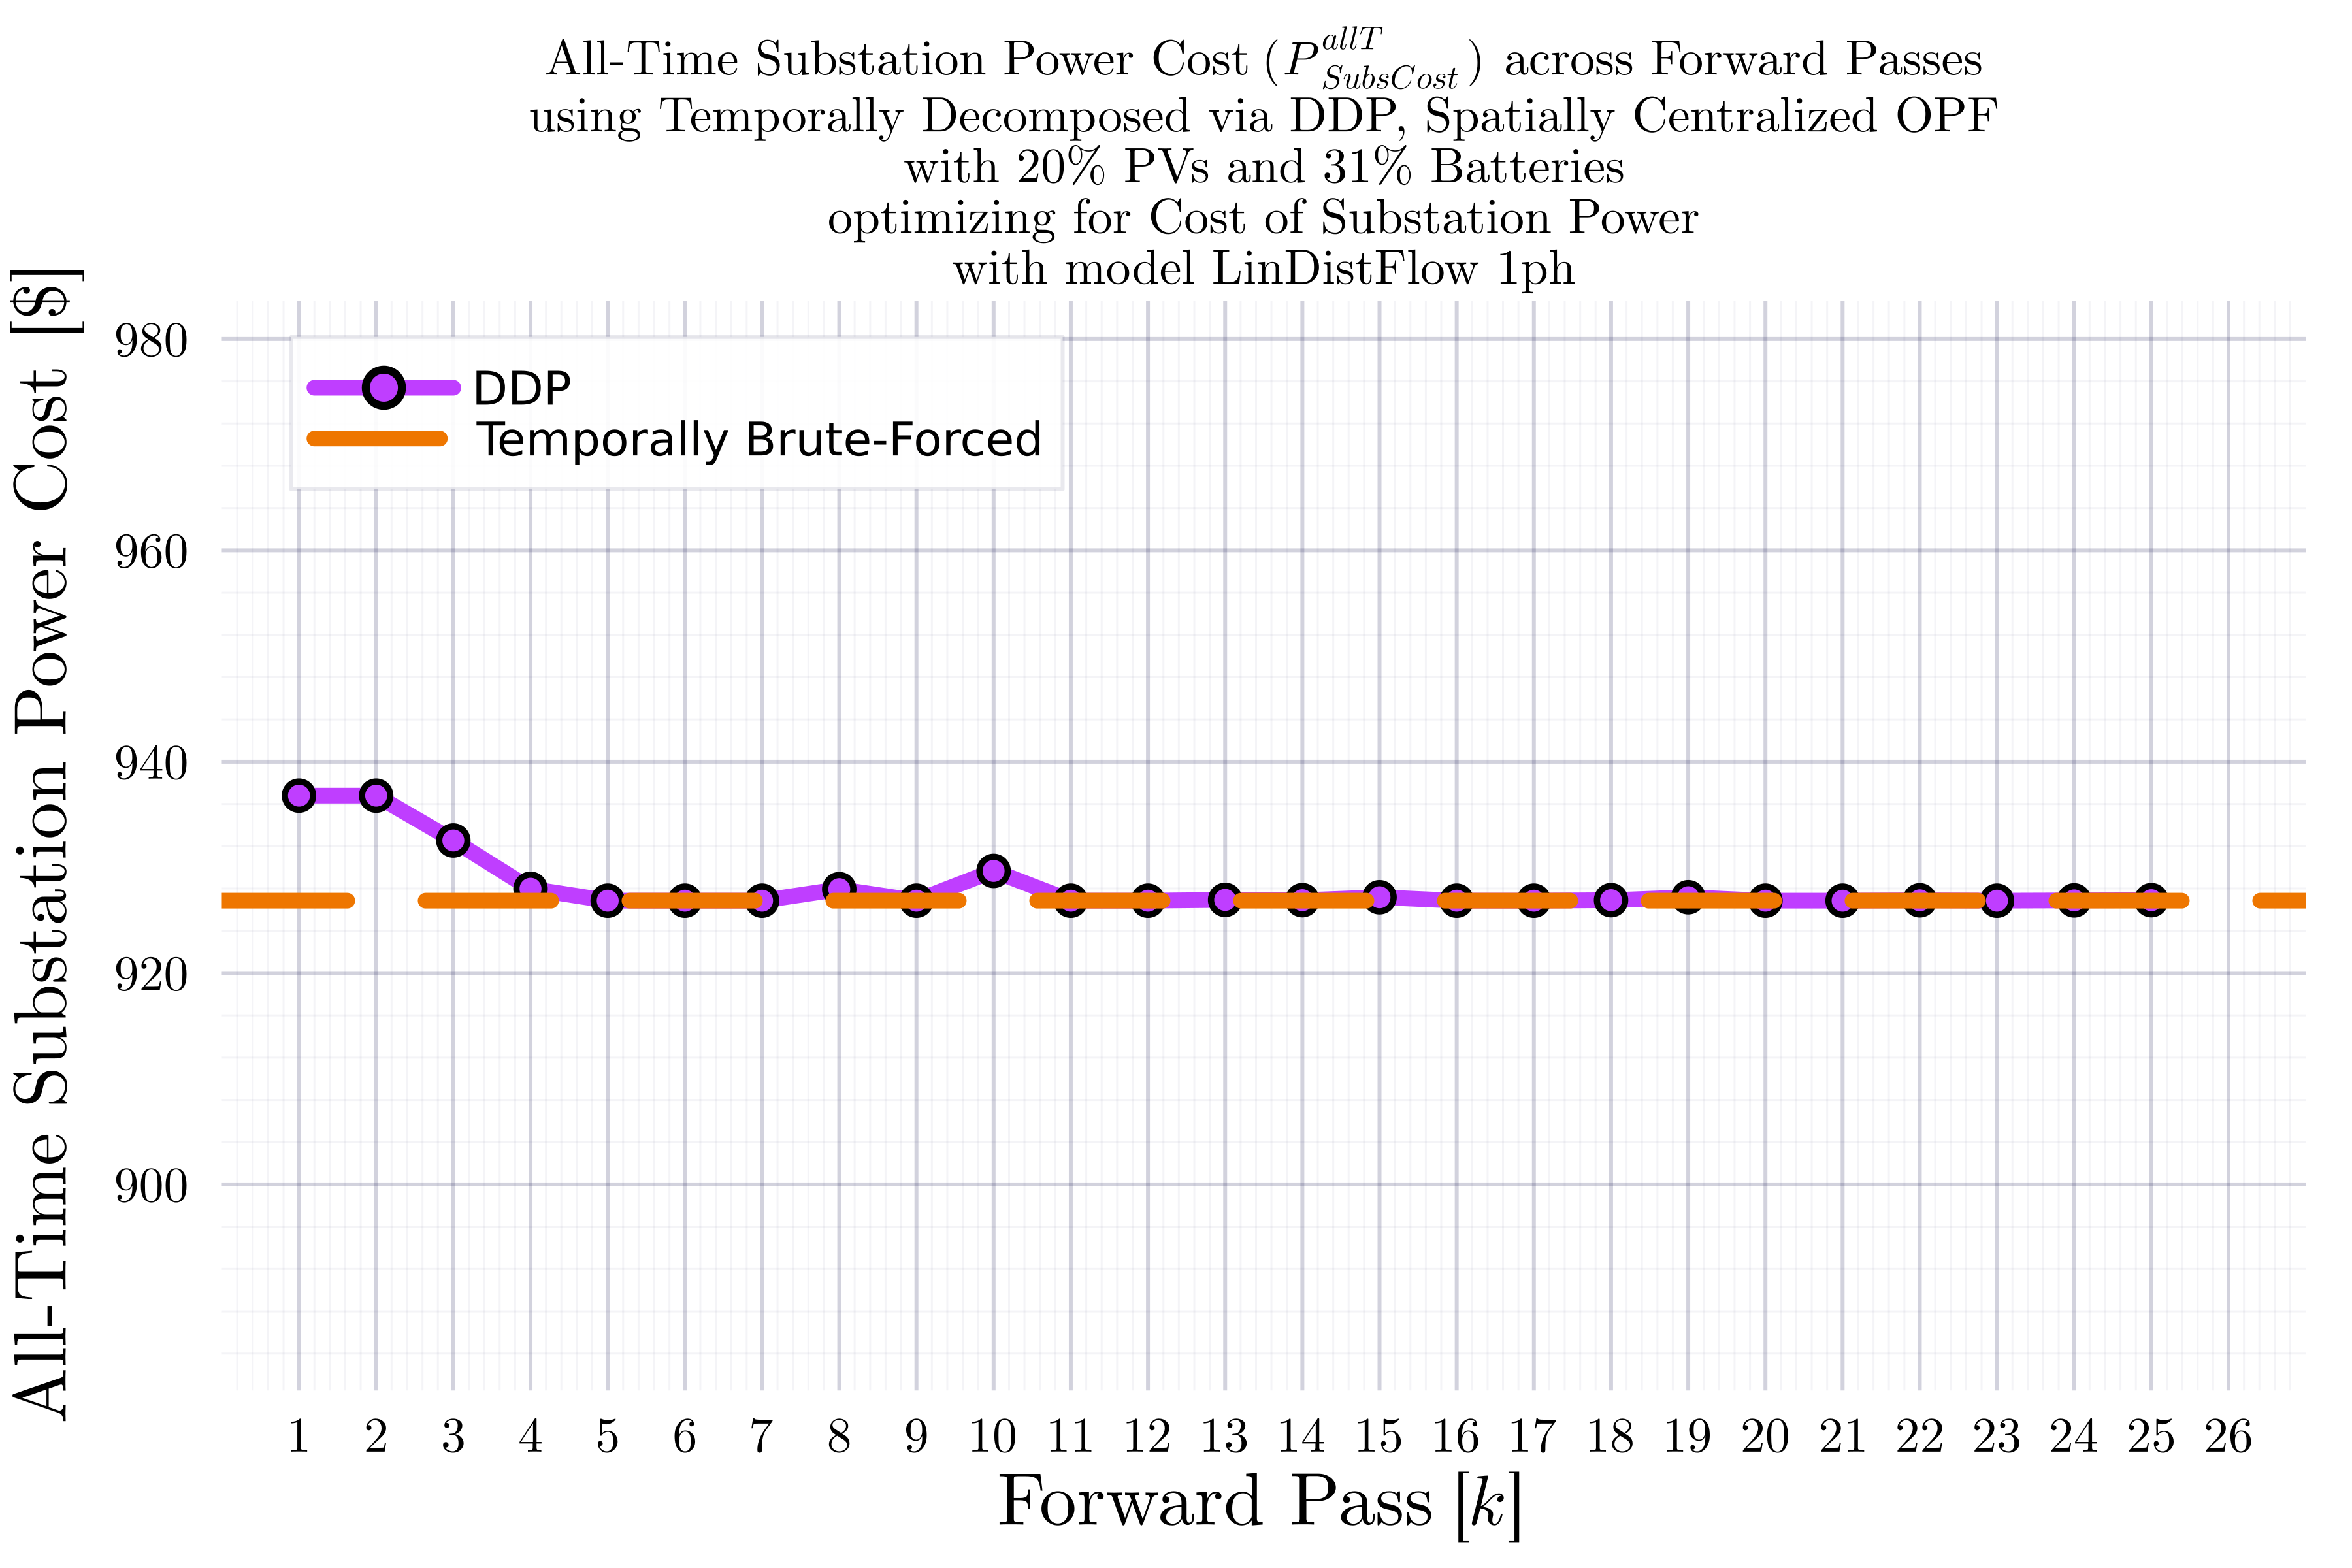
\includegraphics[width=0.85\textwidth]{figures/SubstationPowerCostAllTime_vs_k_26_for_subsPowerCost_min_with_scd_alpha_3_033_gamma_0_0_via_tmprl_dcmpsd_spat_centr_system_with_ldf_1ph.png}
    \caption{All-time substation power cost convergence across forward passes using temporally decomposed DDP with spatially centralized formulation. LinDistFlow model with 20\% PVs and 31\% batteries. Similar rapid convergence observed with the linear model.}
    \label{fig:ddp-convergence-ldf}
\end{figure}

To further validate the robustness of DDP across different loading scenarios, additional tests were performed on a modified IEEE 123-bus variant (ieee123B) with different load profiles. \Cref{fig:ddp-convergence-bfm-b,fig:ddp-convergence-ldf-b} show the convergence behavior for this system configuration.

\begin{figure}[h]
    \centering
    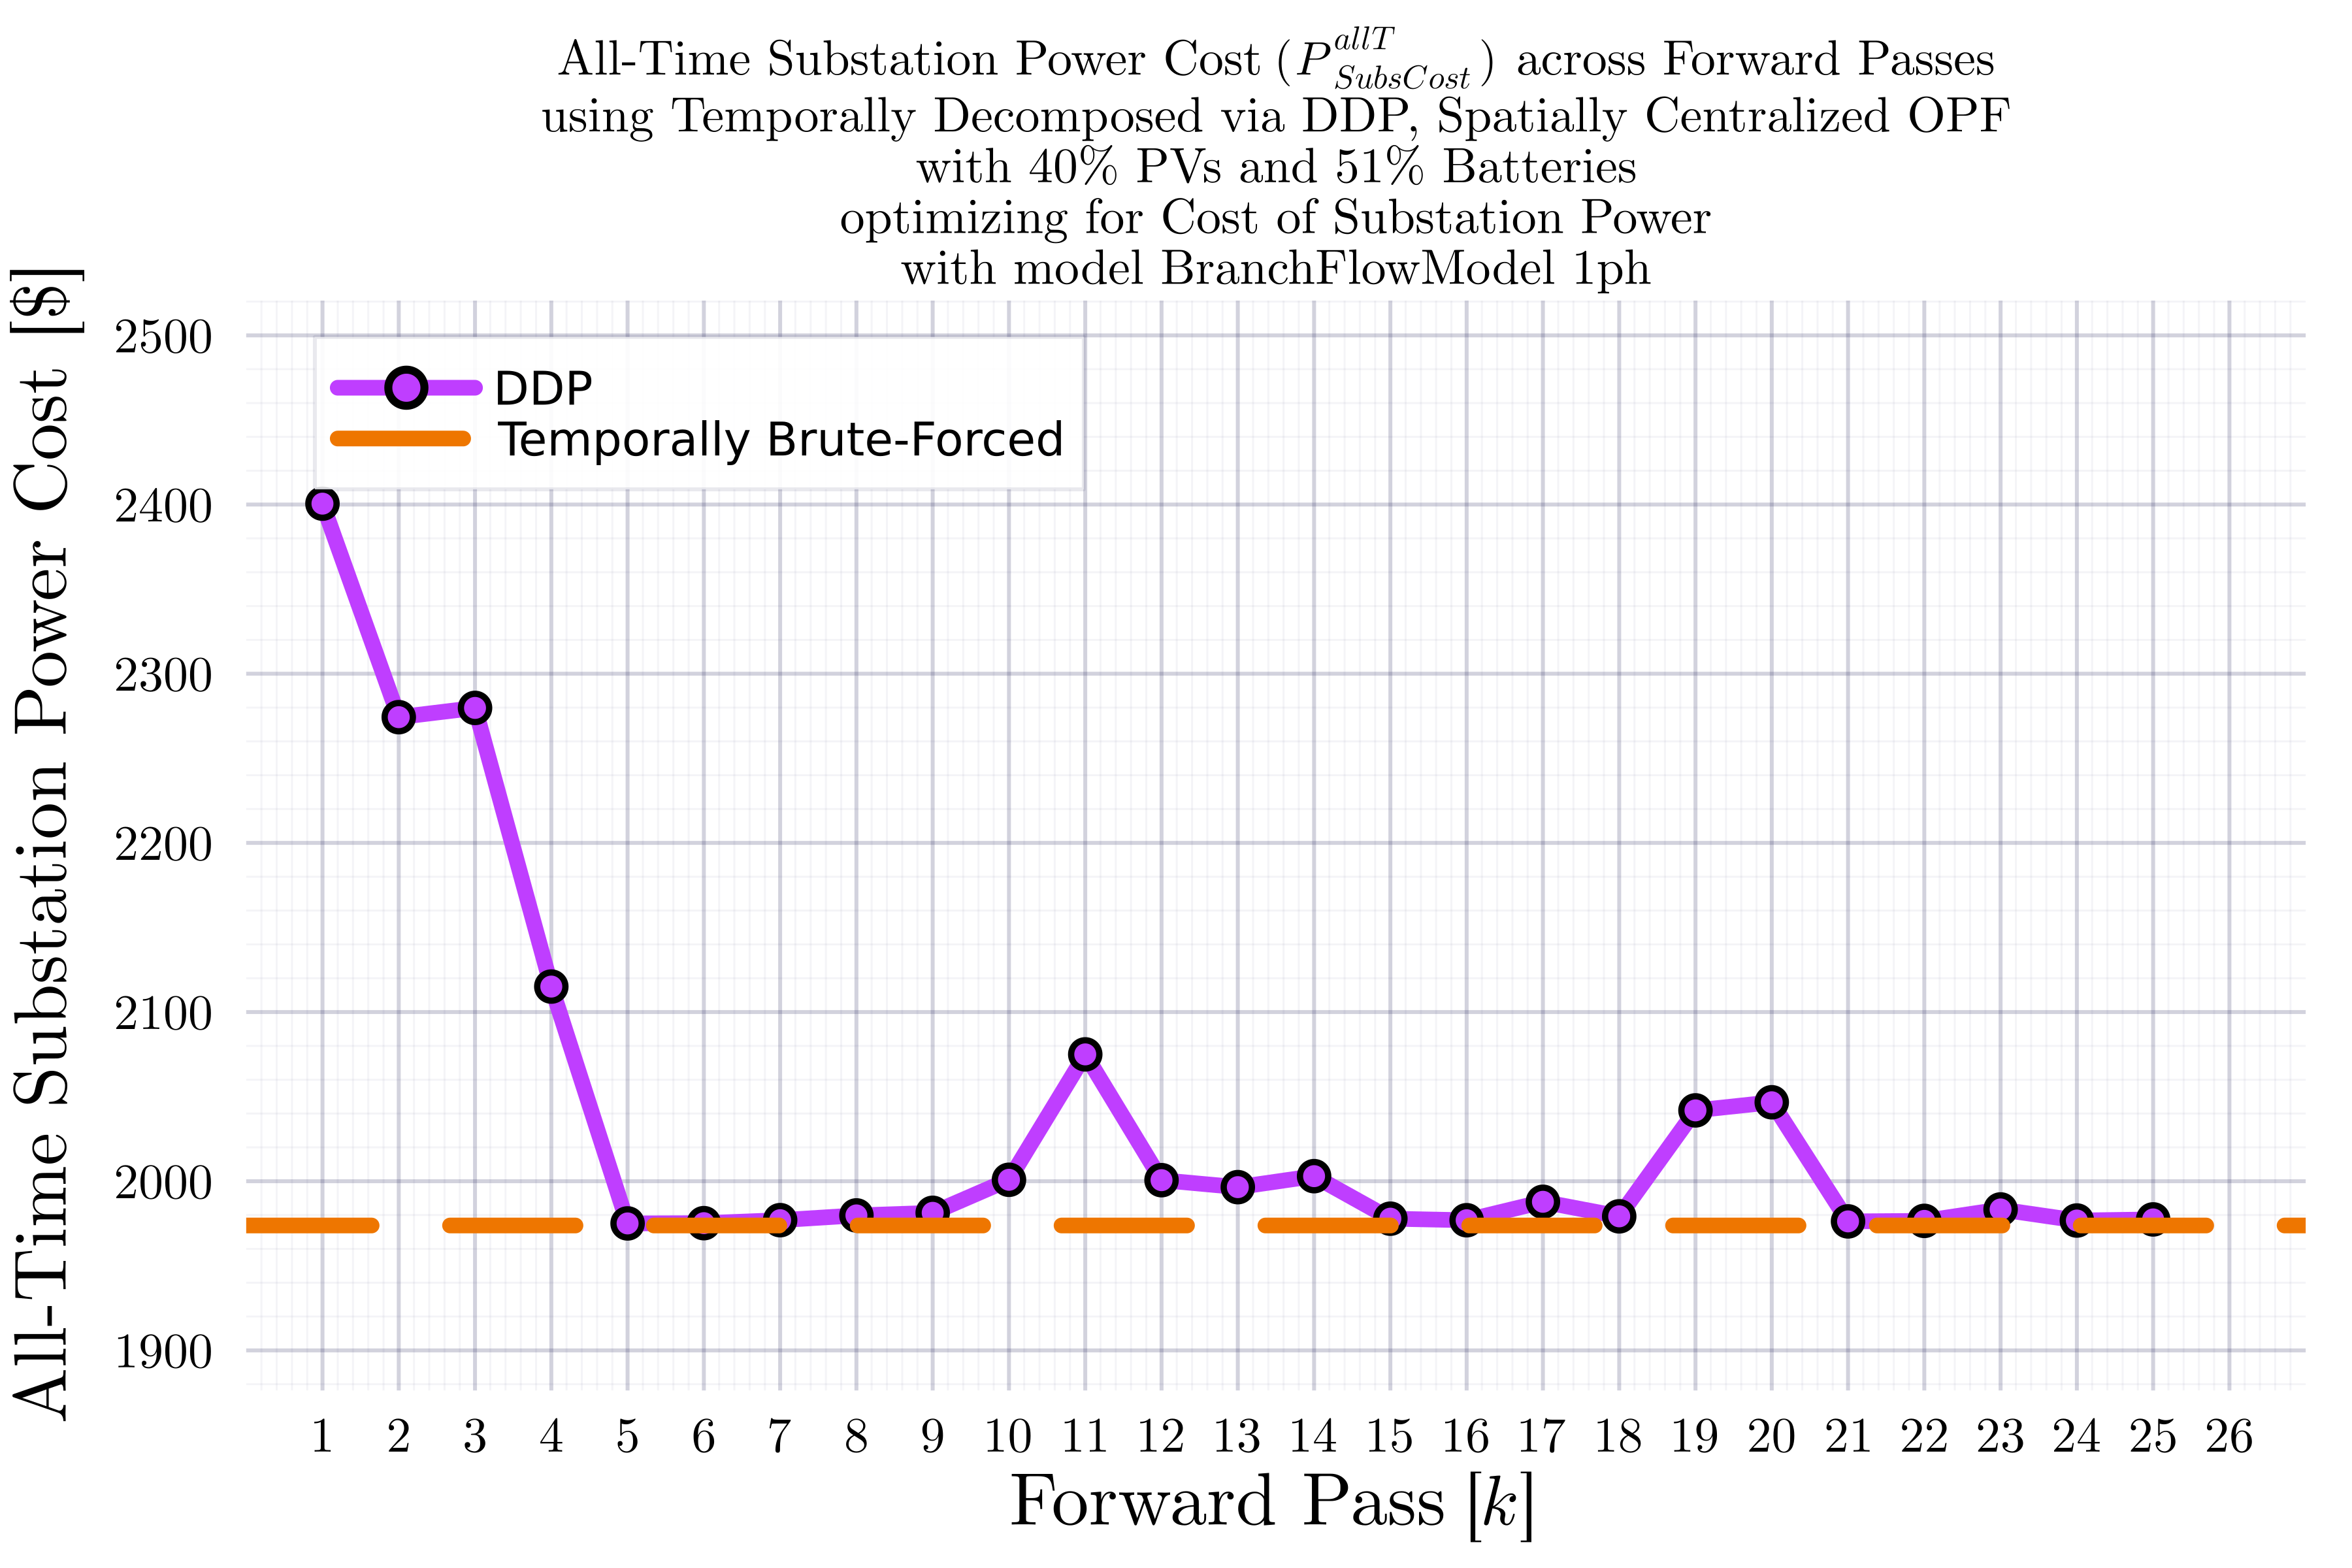
\includegraphics[width=0.85\textwidth]{figures/SubstationPowerCostAllTime_vs_k_26_for_subsPowerCost_min_with_scd_alpha_2_124_gamma_0_0_via_tmprl_dcmpsd_spat_centr_system_with_bfm_NL_1ph.png}
    \caption{All-time substation power cost convergence for ieee123B system using DDP with BFM-NL model. The algorithm exhibits similar rapid convergence characteristics, demonstrating robustness across different system configurations.}
    \label{fig:ddp-convergence-bfm-b}
\end{figure}

\begin{figure}[h]
    \centering
    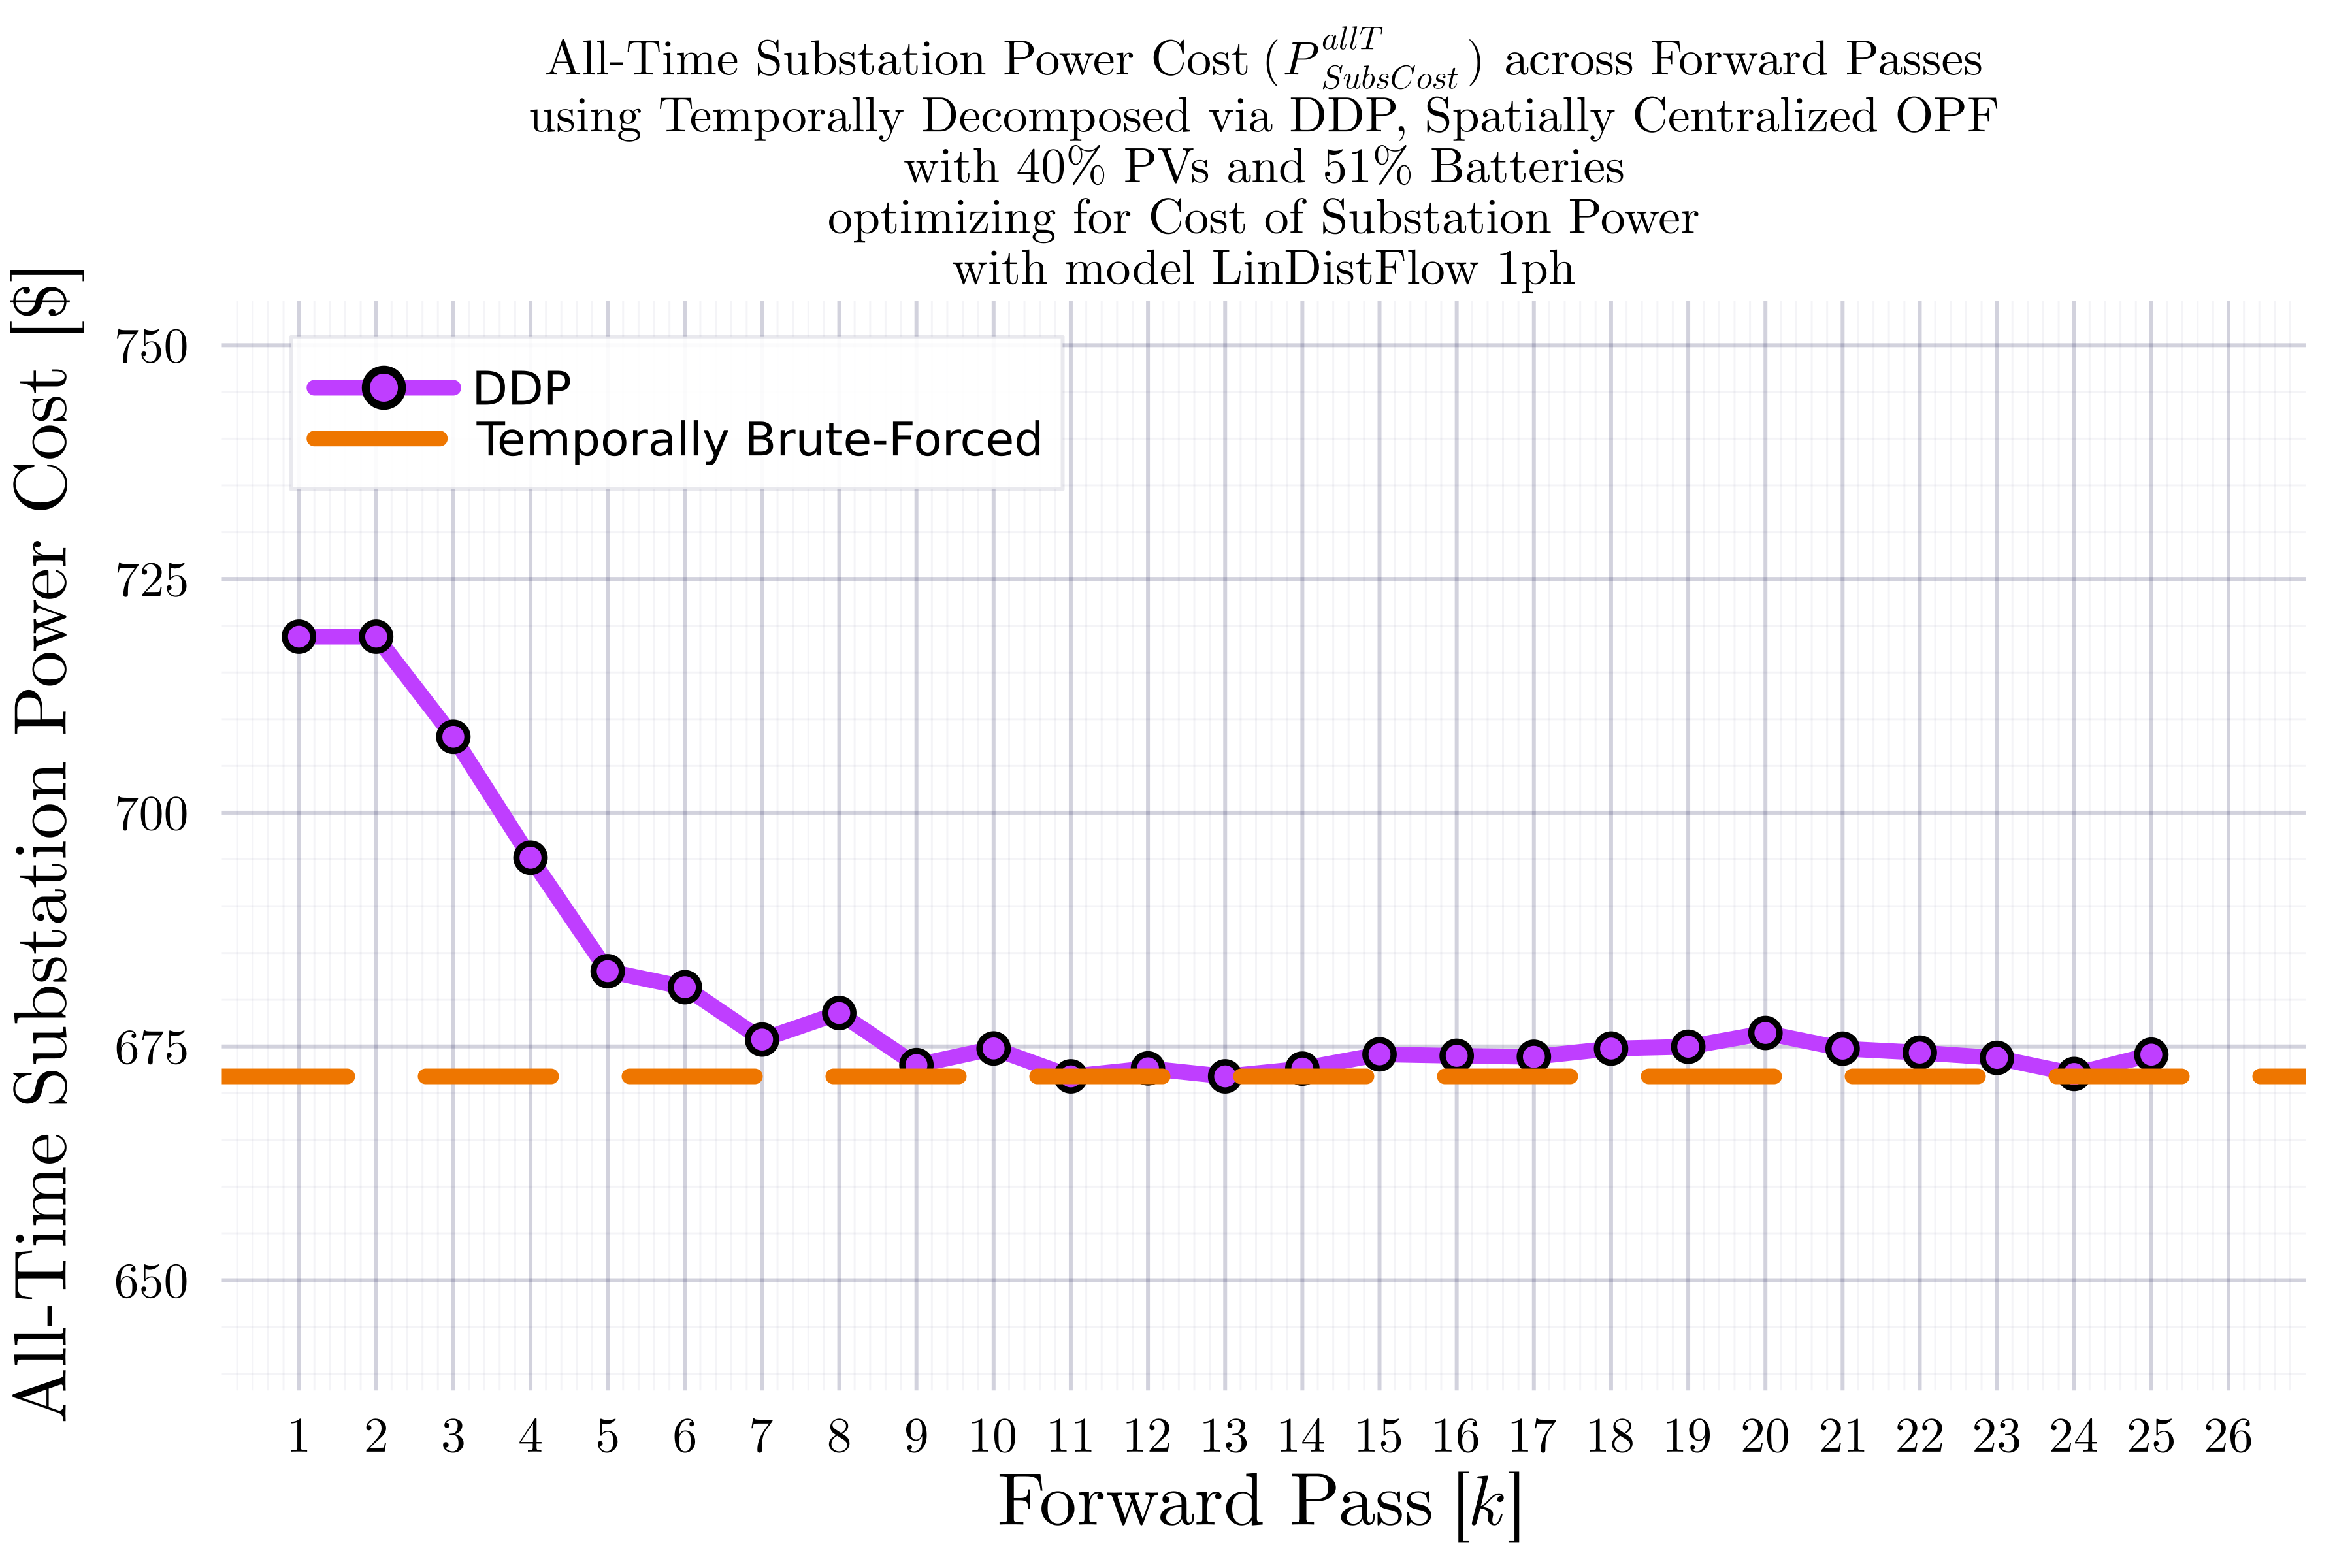
\includegraphics[width=0.85\textwidth]{figures/SubstationPowerCostAllTime_vs_k_26_for_subsPowerCost_min_with_scd_alpha_0_7162_gamma_0_0_via_tmprl_dcmpsd_spat_centr_system_with_ldf_1ph.png}
    \caption{All-time substation power cost convergence for ieee123B system using DDP with LinDistFlow model. Consistent convergence behavior validates DDP's effectiveness across both power flow formulations and system variants.}
    \label{fig:ddp-convergence-ldf-b}
\end{figure}

Key observations from the convergence behavior:
\begin{itemize}
    \item \textbf{Rapid Initial Convergence}: DDP achieves near-optimal cost within 4-5 forward passes, significantly faster than iterative ADMM-based methods
    \item \textbf{Model Independence}: Both BFM-NL and LinDistFlow exhibit similar convergence patterns, validating DDP's applicability across different power flow models
    \item \textbf{System Robustness}: DDP performs consistently well across both ieee123A and ieee123B system variants with different loading profiles, demonstrating robustness to system parameters
    \item \textbf{Optimality Gap}: After convergence, DDP maintains costs very close to the brute-forced (monolithic) solution, with differences less than 0.1\%
\end{itemize}

\subsubsection{Performance Summary}

The final converged solution for ieee123A (after 26 forward passes) achieved the performance metrics summarized in \Cref{tab:ddp-results}. DDP performed similarly well on ieee123B, confirming the algorithm's effectiveness across different system configurations.

\begin{table}[h]
\centering
\caption{DDP Performance Summary for 24-Hour Horizon on IEEE 123-Bus System with 20\% PV and 31\% Battery Penetration (BFM-NL Model, Ipopt Solver)}
\label{tab:ddp-results}
\begin{tabular}{@{}llr@{}}
\toprule
\textbf{Category} & \textbf{Metric} & \textbf{Value} \\ 
\midrule
\multirow{4}{*}{\textbf{Economic \& Power Flow}} 
    & Total Substation Power Cost & \$944.35 \\
    & Total Line Loss & 390.35 kW \\
    & Peak Substation Power & 1,192.95 kW \\
    & Total Substation Power & 21,022.04 kW + 7,232.8 kVAr \\
\midrule
\multirow{4}{*}{\textbf{DER Performance}} 
    & PV Generation (Total) & 607.46 kW + 1,972.4 kVAr \\
    & Battery Net Discharge & 118.29 kW + 3,310.45 kVAr \\
    & Battery Transaction Magnitude & 1,034.31 kW \\
    & Final SOC Deviation from Reference & 171.32 kWh \\
\midrule
\multirow{3}{*}{\textbf{Solution Quality}} 
    & Maximum Voltage Discrepancy & 0.000759 pu \\
    & Maximum Line Loss Discrepancy & 13.15 kW \\
    & Maximum Substation Power Discrepancy & 13.10 kW, 14.48 kVAr \\
\bottomrule
\end{tabular}
\end{table}

Key observations from \Cref{tab:ddp-results}:
\begin{itemize}
    \item \textbf{High Accuracy}: Voltage discrepancies below 0.08\% and power discrepancies less than 1\% of peak power validate the solution quality
    \item \textbf{Effective DER Coordination}: Batteries perform significant transactions (1,034 kW total) while maintaining reasonable final SOC deviation
    \item \textbf{Computational Efficiency}: Achieving these results through temporal decomposition enables scalability to longer horizons
\end{itemize}

\subsubsection{Preliminary Results on Larger Systems}

To explore DDP's scalability to larger distribution networks, preliminary tests were conducted on the IEEE 730-bus system. \Cref{fig:ddp-convergence-ieee730} shows the convergence behavior using LinDistFlow with relaxed convergence criteria (function value-based termination).

\begin{figure}[h]
    \centering
    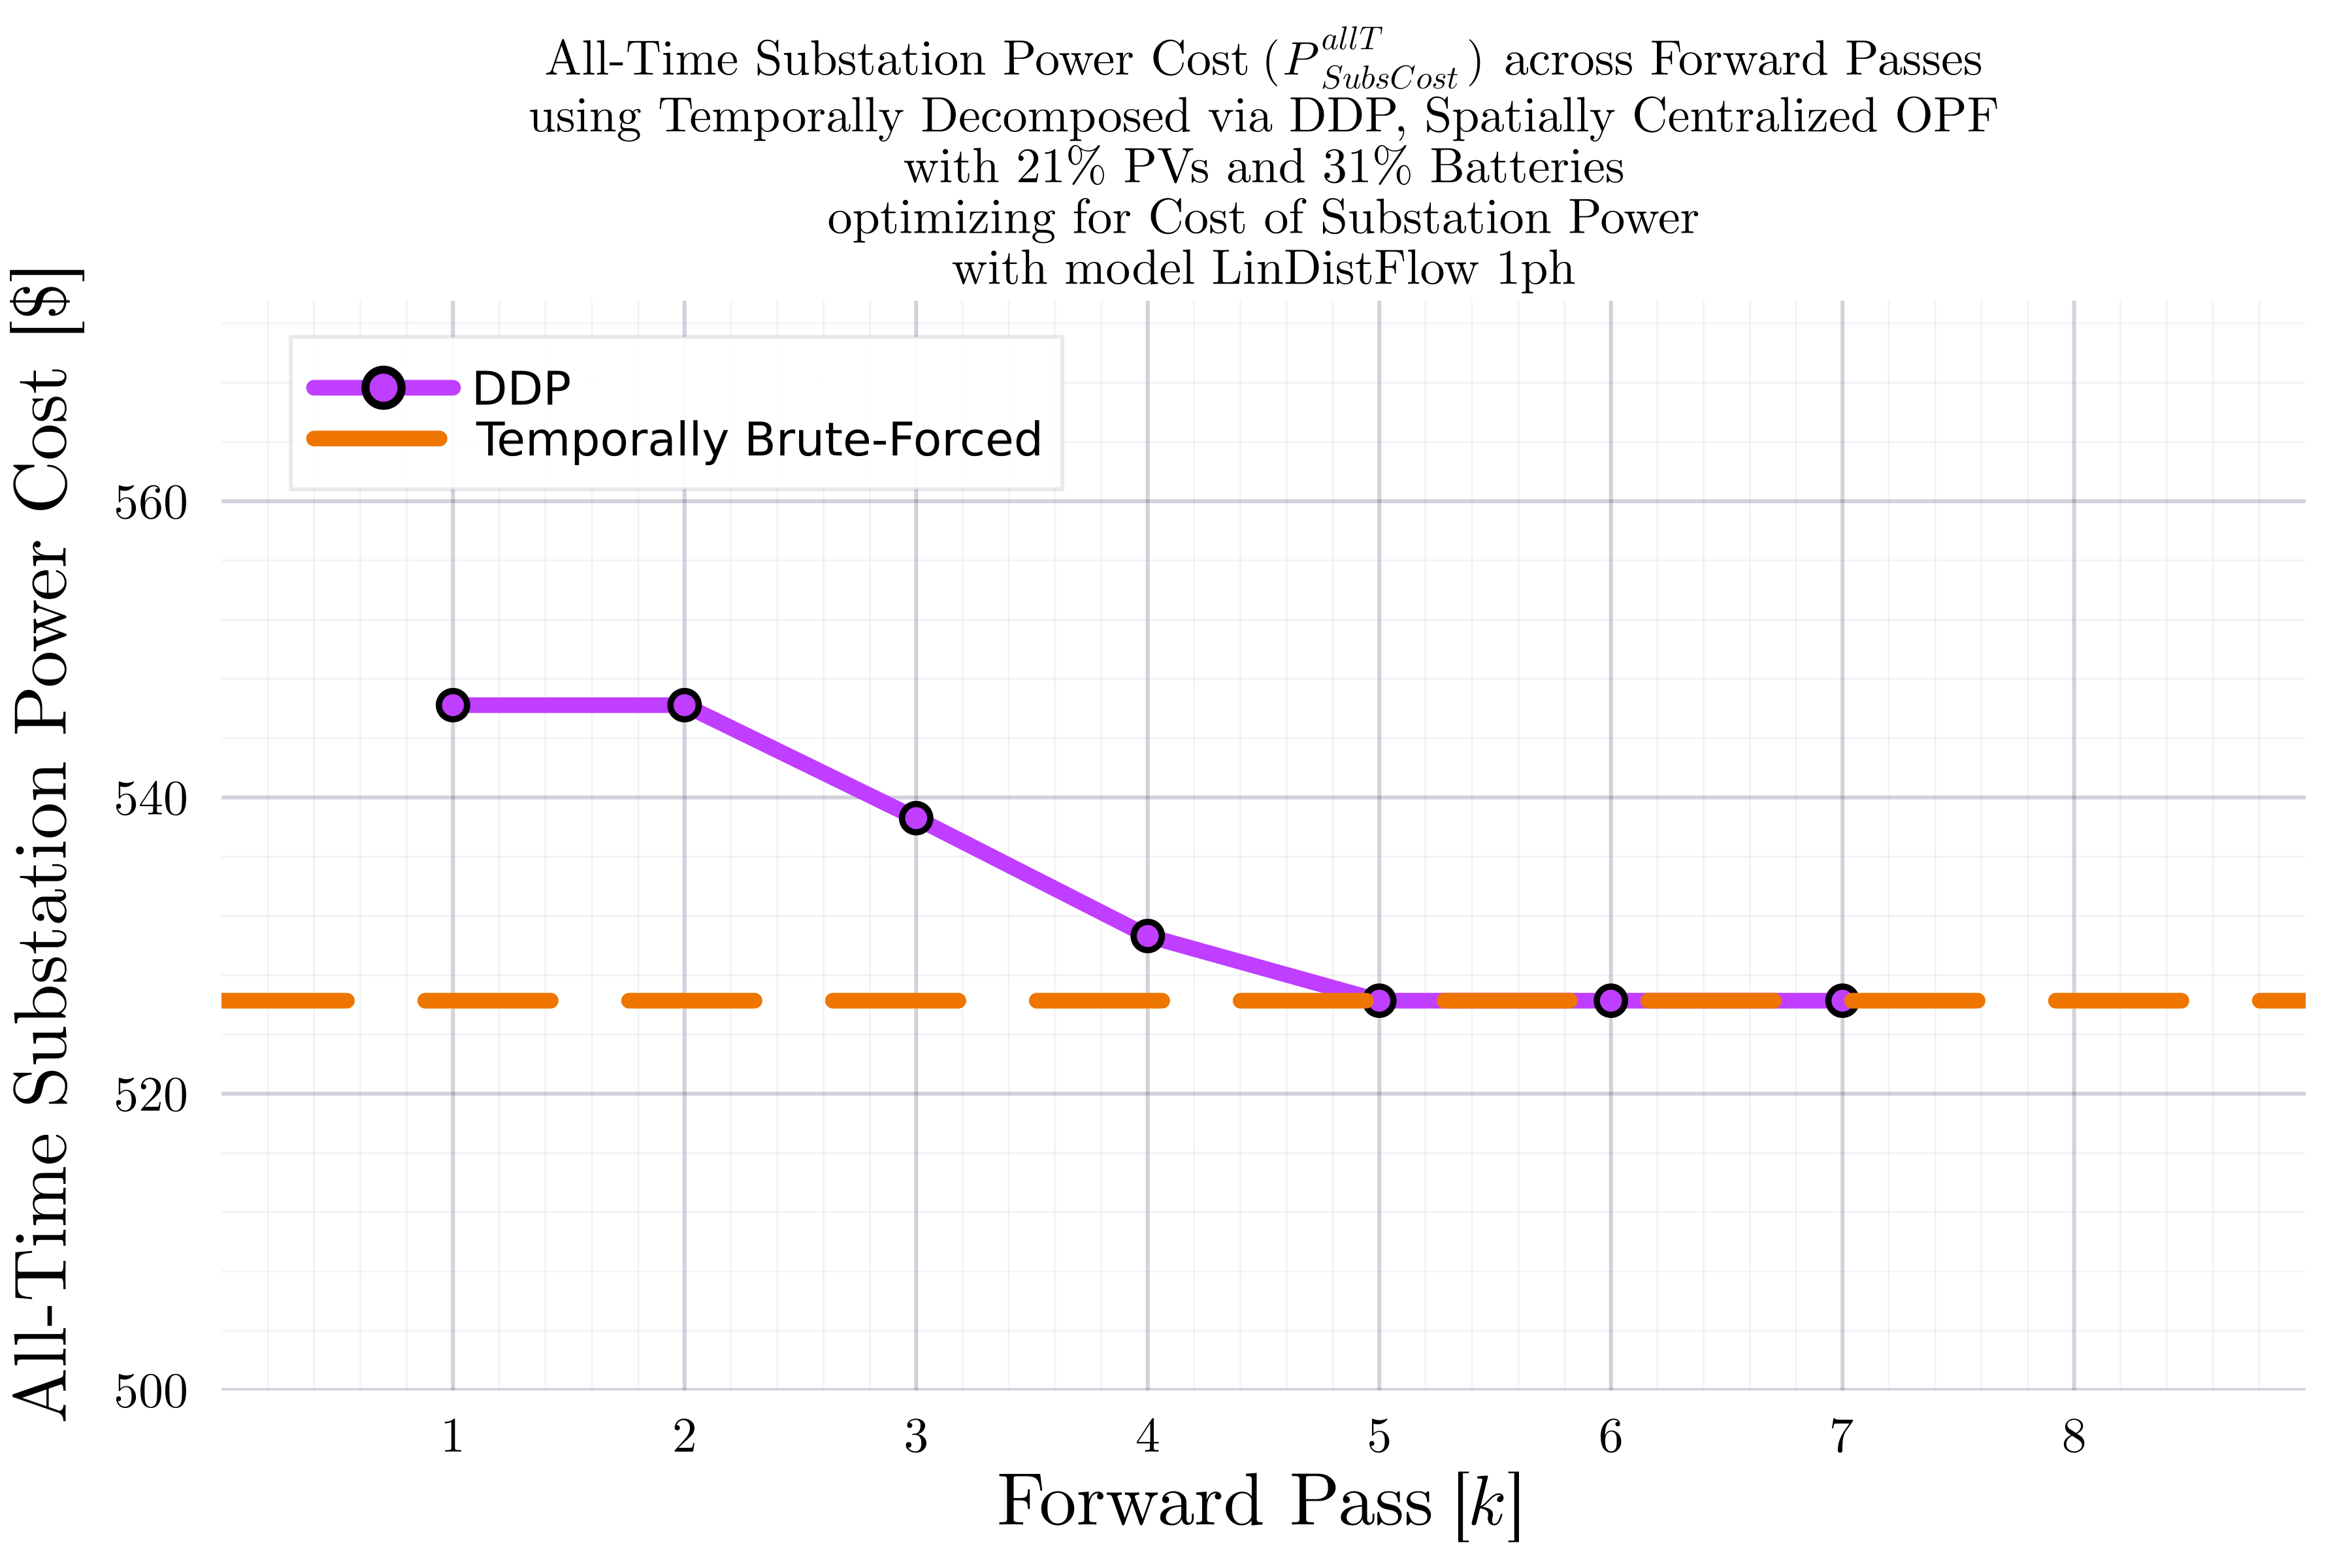
\includegraphics[width=0.85\textwidth]{figures/SubstationPowerCostAllTime_vs_k_8_for_subsPowerCost_min_with_scd_alpha_1_08_gamma_0_0_via_tmprl_dcmpsd_spat_centr_system_with_ldf_1ph.png}
    \caption{All-time substation power cost convergence for IEEE 730-bus system using DDP with LinDistFlow model. The algorithm shows directional convergence toward the optimal solution, though requiring relaxed termination criteria. Results indicate DDP's potential for large-scale systems while highlighting areas for algorithmic refinement.}
    \label{fig:ddp-convergence-ieee730}
\end{figure}

While the results in \Cref{fig:ddp-convergence-ieee730} demonstrate that DDP's optimization trajectory is moving in the right direction, the convergence behavior suggests that further research is needed to:
\begin{itemize}
    \item \textbf{Enhance Convergence Rigor}: Develop more robust stopping criteria and regularization strategies for larger systems
    \item \textbf{Scale Initialization}: Develop better warm-start strategies that leverage system structure for networks with 500+ buses
\end{itemize}

These preliminary findings indicate that while DDP shows promise for temporal decomposition of large-scale MPOPF problems, additional algorithmic development is necessary to achieve an adequate level of  convergence reliability. This represents an important direction for future work.

%%%%%%%%%%%%%%%%%%%%%%%%%%%%%%%%%%%%%%%%%%%%%%%%%%%%%%%%%%%%%%%%%%%%%%%%
\subsection{Summary}
%%%%%%%%%%%%%%%%%%%%%%%%%%%%%%%%%%%%%%%%%%%%%%%%%%%%%%%%%%%%%%%%%%%%%%%%

Differential Dynamic Programming provides a principled temporal decomposition framework for large-scale MPOPF problems. By reformulating MPOPF as an optimal control problem with battery SOC as states, DDP achieves:

\begin{itemize}
    \item \textbf{Linear time complexity} $\mathcal{O}(N)$ in horizon length $N$
    \item \textbf{Natural handling} of nonlinear branch flow models (BFM-NL) without approximation
    \item \textbf{Sequential structure} exploiting causal battery dynamics
    \item \textbf{Warm-start capability} for rolling-horizon MPC implementations
\end{itemize}

The key insight is that battery SOC couples time periods, while power flow constraints decouple across time. DDP leverages this structure by solving backward-forward passes, where:
\begin{itemize}
    \item \textbf{Backward pass}: Computes optimal feedback policy (how battery should react to SOC deviations)
    \item \textbf{Forward pass}: Rolls out trajectory respecting power flow constraints at each time step
\end{itemize}

The next chapter explores an alternative temporal decomposition approach based on ADMM consensus, which trades off its sequential nature for parallelizability and convex convergence guarantees.
